\documentclass{article}


%%%%
% PLOTS mapas y conglomerados
% bibliografia
%%%%
\usepackage[utf8]{inputenc}
\usepackage{longtable}
\usepackage{authblk}
\usepackage{adjustbox}

\usepackage{natbib}



\title{INDICES POBLACIONALES EN COLOMBIA POR DEPARTAMENTO}
% autores

\author[]{\normalsize Lorenzo Vicini}



\affil[1,2]{\small  Escuela de Ingenieria,Universidad de los Andes\\
\texttt{{Herramientas Computacionales} le.vicini10@uniandes.edu.co}}
\date{02 de Julio de 2018}
%%%%




\usepackage{Sweave}
\begin{document}

\Sconcordance{concordance:Proyecto1111.tex:Proyecto1111.Rnw:%
1 31 1 1 0 23 1 1 8 1 1 1 5 15 0 1 2 1 1 1 5 1 3 3 1 1 6 2 1 1 5 1 2 6 %
1 1 4 12 0 1 2 4 1 1 17 13 0 1 7 1 1 1 3 1 2 12 1 1 15 31 0 1 2 12 1 1 %
15 1 14 1 1 1 18 1 2 5 1}

\maketitle
\begin{abstract}
Este es mi primer trabajo en exploracion y modelamiento de indices usando LATEX. Este trabajo lo he hecho bajo la filosofia de trabajo replicable a partir de el archivo provisto por el profesor del curso, el cual hacia uso de programas tales como: RStudio, Python, Zotero, entre otros.\cite{macqueen_methods_nodate}
\end{abstract}

\section*{Introduccion}

El siguiente trabajo pretende mostrar El indice de desarrollo humano (IDH) para Colombia a partir de la densidad poblacional de cada departamento, la cual se divide en rural y urbana. Cabe recordar que el IDH  es un indicador del desarrollo humano por pais, elaborado por el Programa de las Naciones Unidas para el Desarrollo , el cual tiene en cuenta: el tener una vida larga y saludable, adquirir conocimientos, esperanza de vida, periodos de educacion recibidos, indice del PIB, etc.  
En el desarrollo del trabajo se realizaran analisis estadisticos fundamentados con graficas y tablas. Se finalizara con un analisis de Clusterizacion el cual mostrara de manera grafica el desarrollo de los diferentes departamentos de Colombia. 

\clearpage


\section{Exploracion Univariada}\label{univariada}

Se denomina exploracion univariada al proceso en el que se obtiene las medidas estadisticas, la tabla de frecuencias y algun grafico de resumen de una variable en particular.Dichos datos  y analisis se mostraran acontinuacion. En esta seccion se exploran los diferentes datos  (IDH, Poblacion Rural y Urbana) 

Comencemos viendo que hay en la sección \ref{univariada} en la página \pageref{univariada}.





% Table created by stargazer v.5.2.2 by Marek Hlavac, Harvard University. E-mail: hlavac at fas.harvard.edu
% Date and time: mar., jul. 03, 2018 - 8:49:57 p. m.
\begin{table}[!htbp] \centering 
  \caption{Medidas estadisticas} 
  \label{stats} 
\begin{tabular}{@{\extracolsep{5pt}}lcc} 
\\[-1.8ex]\hline 
\hline \\[-1.8ex] 
Statistic & \multicolumn{1}{c}{N} & \multicolumn{1}{c}{Median} \\ 
\hline \\[-1.8ex] 
IDH & 32 & 0.804 \\ 
Población.Cabecera & 32 & 717,197 \\ 
Población.Resto & 32 & 268,111.5 \\ 
Población.Total & 32 & 1,028,429 \\ 
\hline \\[-1.8ex] 
\end{tabular} 
\end{table} \begin{figure}[h]

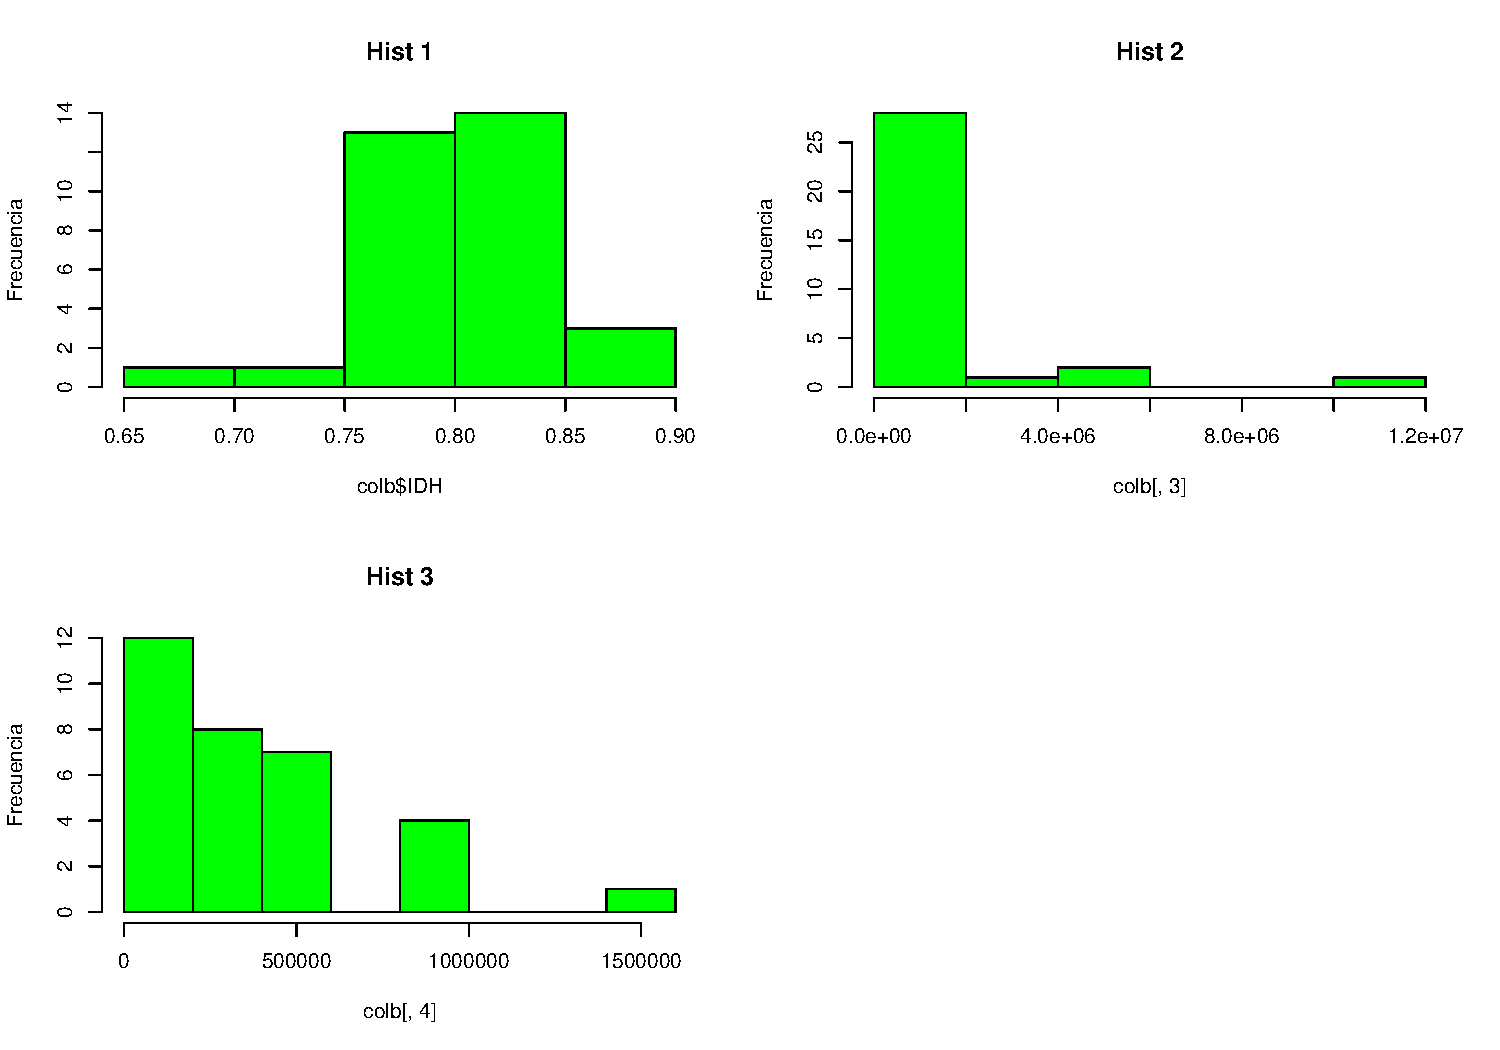
\includegraphics{Proyecto1111-hist}

\caption{Histogramas Iniciales}
\label{F1}
\end{figure}


\begin{figure}[h]
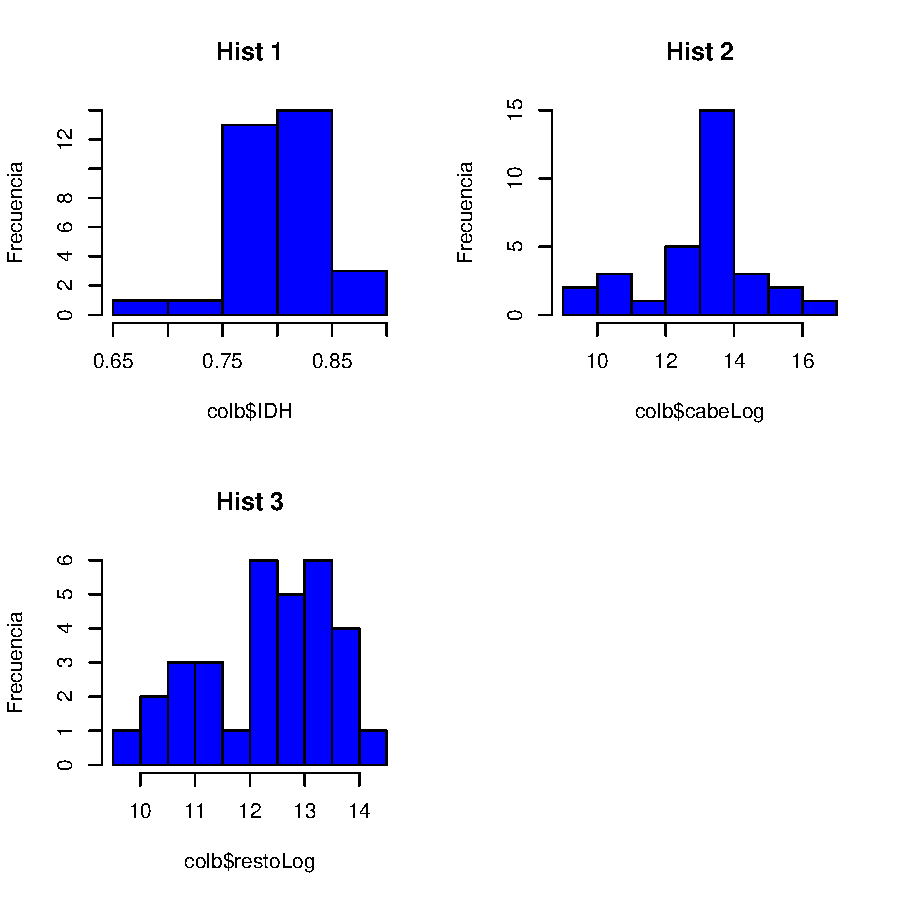
\includegraphics{Proyecto1111-log}
\caption{Histogramas despues de la transformacion logaritmica}
\end{figure}
\clearpage

\section{Exploracion Bivariada}
 Las correlaciones bivariadas son herramientas comunes y se utilizan para estudiar como una variable influye con otra. En esta seccion se genera un analisis de la variable IDH con respecto a las otras dos variables (poblacion urabana y rural)

% Table created by stargazer v.5.2.2 by Marek Hlavac, Harvard University. E-mail: hlavac at fas.harvard.edu
% Date and time: mar., jul. 03, 2018 - 8:50:02 p. m.
\begin{table}[!htbp] \centering 
  \caption{Correlacion de IDH con las demas variables} 
  \label{corrDem} 
\begin{tabular}{@{\extracolsep{5pt}} cc} 
\\[-1.8ex]\hline 
\hline \\[-1.8ex] 
cabeLog & restoLog \\ 
\hline \\[-1.8ex] 
$0.487$ & $0.177$ \\ 
\hline \\[-1.8ex] 
\end{tabular} 
\end{table} 
En probabilidad y estadistica, la correlacion indica la fuerza y la direccion de una relacion lineal y proporcionalidad entre dos variables estadisticas. Se considera que dos variables cuantitativas estan correlacionadas cuando los valores de una de ellas varian sistematicamente con respecto a los valores de la otra. 

Estos son los resultados de la correlacion: 

% Table created by stargazer v.5.2.2 by Marek Hlavac, Harvard University. E-mail: hlavac at fas.harvard.edu
% Date and time: mar., jul. 03, 2018 - 8:50:02 p. m.
\begin{table}[!htbp] \centering 
  \caption{Correlación entre variables independientes} 
  \label{corrTableX} 
\begin{tabular}{@{\extracolsep{5pt}} ccc} 
\\[-1.8ex]\hline 
\hline \\[-1.8ex] 
 & cabeLog & restoLog \\ 
\hline \\[-1.8ex] 
cabeLog & 1 &  \\ 
restoLog & 0.84 & 1 \\ 
\hline \\[-1.8ex] 
\end{tabular} 
\end{table} 
\begin{figure}[h]
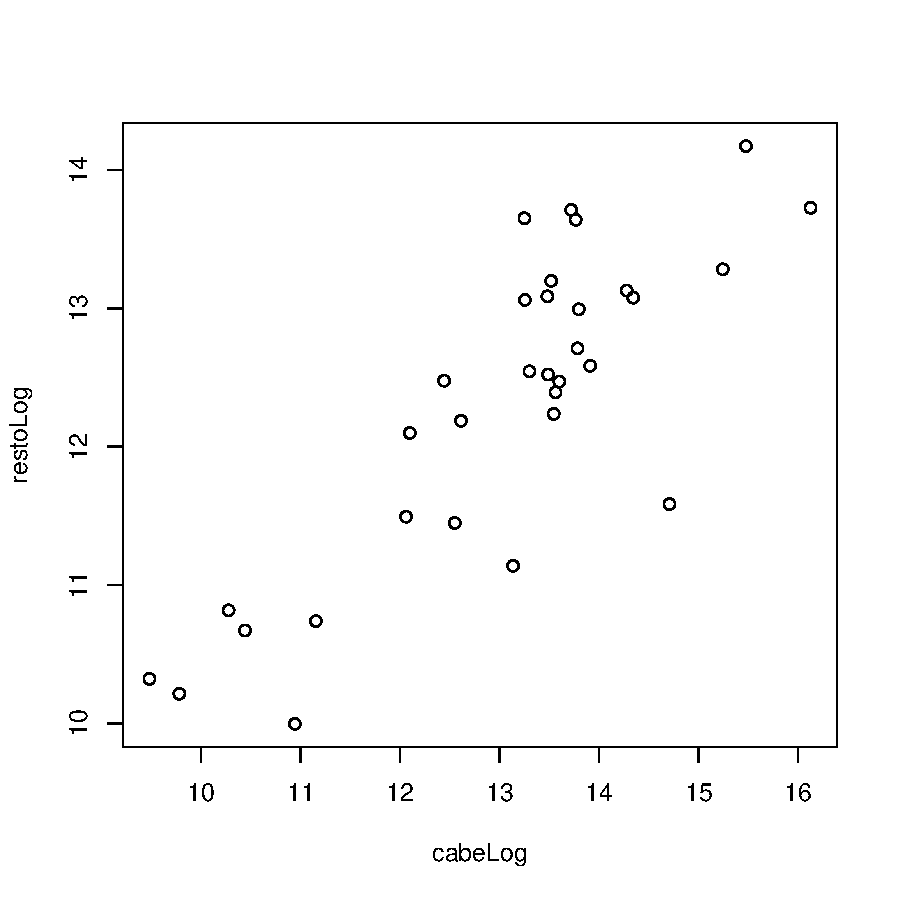
\includegraphics{Proyecto1111-grafico}
\caption{Grafico de dispersion}
\end{figure}



\clearpage

\section{Modelos de Regresion}



En estadistica, el analisis de la regresion es un proceso estadistico para estimar las relaciones entre variables. Incluye muchas tecnicas para el modelado y analisis de diversas variables, cuando la atencion se centra en la relacion entre una variable dependiente y una o mas variables independientes. Para nuestro caso, la variable dependiente sera el IDH.  

% Table created by stargazer v.5.2.2 by Marek Hlavac, Harvard University. E-mail: hlavac at fas.harvard.edu
% Date and time: mar., jul. 03, 2018 - 8:50:02 p. m.
\begin{table}[!htbp] \centering 
  \caption{Modelos de Regresi<f3>n} 
  \label{regresiones} 
\begin{tabular}{@{\extracolsep{5pt}}lcc} 
\\[-1.8ex]\hline 
\hline \\[-1.8ex] 
 & \multicolumn{2}{c}{\textit{Dependent variable:}} \\ 
\cline{2-3} 
\\[-1.8ex] & \multicolumn{2}{c}{IDH} \\ 
\\[-1.8ex] & (1) & (2)\\ 
\hline \\[-1.8ex] 
 cabeLog & 0.013$^{***}$ & 0.031$^{***}$ \\ 
  & (0.004) & (0.007) \\ 
  & & \\ 
 restoLog &  & $-$0.030$^{***}$ \\ 
  &  & (0.010) \\ 
  & & \\ 
 Constant & 0.634$^{***}$ & 0.766$^{***}$ \\ 
  & (0.055) & (0.065) \\ 
  & & \\ 
\hline \\[-1.8ex] 
Observations & 32 & 32 \\ 
R$^{2}$ & 0.238 & 0.425 \\ 
Adjusted R$^{2}$ & 0.212 & 0.385 \\ 
Residual Std. Error & 0.037 (df = 30) & 0.033 (df = 29) \\ 
F Statistic & 9.347$^{***}$ (df = 1; 30) & 10.706$^{***}$ (df = 2; 29) \\ 
\hline 
\hline \\[-1.8ex] 
\textit{Note:}  & \multicolumn{2}{r}{$^{*}$p$<$0.1; $^{**}$p$<$0.05; $^{***}$p$<$0.01} \\ 
\end{tabular} 
\end{table} 


\clearpage




\section{Exploracion Espacial}

Para realizar el siguiente mapa, se llevo a cabo la utilizacion de la tecnica de "Kmeans" la cual es un metodo de agrupamiento, que tiene como objetivo la particion de un conjunto de n observaciones en k grupos en el que cada observacion pertenece al grupo cuyo valor medio es mas cercano.Lo cual realizaremos con el mapa de Colombia para mostrar de manera grafica el desarrollo de cada departamento clasificado en tres categorias: Alto, medio y bajo. 





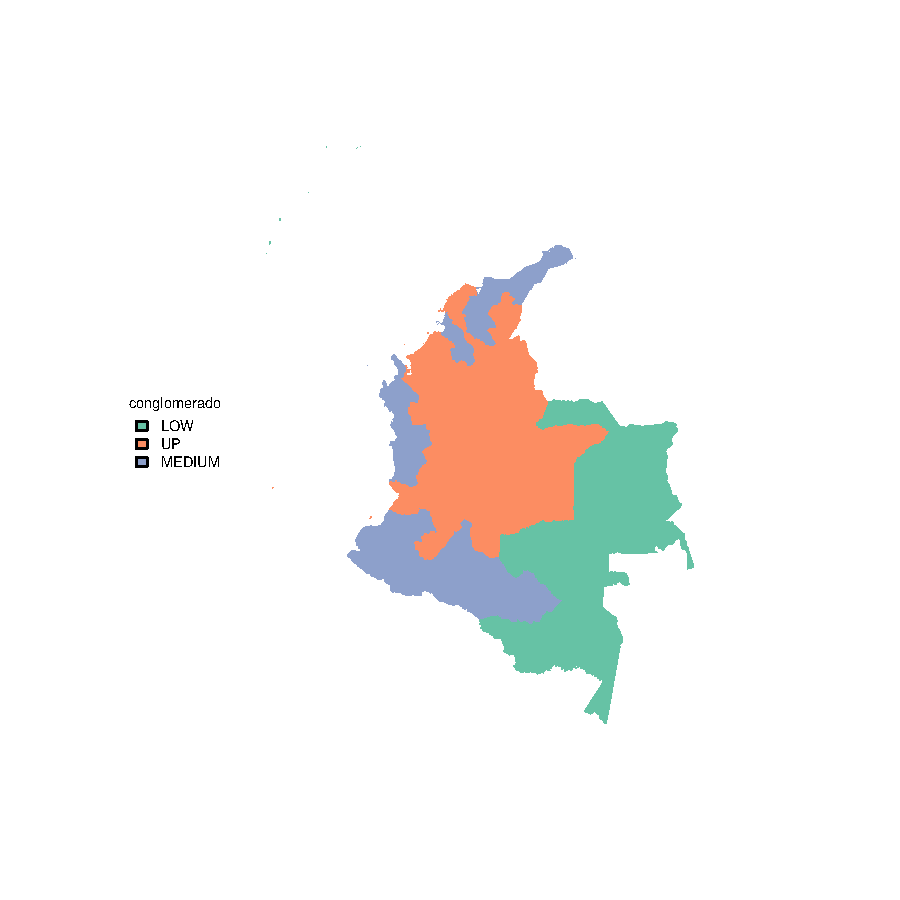
\includegraphics{Proyecto1111-plotMap1}

\bibliographystyle{abbrv}
\renewcommand{\refname}{Bibliografia}
\bibliography{ProyectoZotero}

\end{document}
